\chapter{Rendering}
\label{chapter render}
In computer graphics applications, the ultimate goal for fluid simulation is usually so that the fluid can be rendered and displayed to the human user. Thus, in addition to the FLIP and PBF algorithm, this project also implements a rendering pipeline, so that the simulation and rendering and be conducted together in real time. This chapter introduces the key rendering facilities that are implemented and the algorithms used.

\section{Surface Reconstruction}
\label{section surface reconstruction}
To render liquids, the first step is to represent the surface of the liquid as a mesh of triangles, which can then be fed into the GPU rendering pipeline. Since this triangle mesh is not maintained by the simulation algorithms, it needs to be generated in each frame. Fortunately, both FLIP and PBF maintains a cloud of particles that occupy the entire fluid region, so if an algorithm can reconstruct a triangle mesh from particles, it can be used to render the results of both simulation algorithms.

In the paper where they also described FLIP\cite{zhu2005animating}, Zhu and Bridson utilized a concept called \textit{Signed Distance Field} to perform surface reconstruction. The signed distance field $\phi : \mathbb{R} ^3 \rightarrow \mathbb{R}$  is a scalar field, with the property that, given a 3D cartesian coordinate $\textbf{x}$:
\begin{itemize}
    \item $\phi(\textbf{x}) = 0$ if $\textbf{x}$ is on the boundary of the fluid region.
    
    \item $\phi(\textbf{x}) = d$ if $\textbf{x}$ is outside the fluid region, and the shortest distance between $\textbf{x}$ and any point on the surface is $d$.
    
    \item $\phi(\textbf{x}) = -d$ if $\textbf{x}$ is inside the fluid region, and the shortest distance between $\textbf{x}$ and any point on the surface is $d$.
\end{itemize}
Thus, the magnitude of $\phi(\textbf{x})$ indicates the distance between $\textbf{x}$ and the surface, and the sign of $\phi(\textbf{x})$ indicates whether $\textbf{x}$ is in the inside or outside. The fluid surface is then precisely the set of points where $\phi$ evaluates to 0. In literature, this is often called the \textit{zero isocontour} or \textit{zero isosurface}.

Zhu and Bridson's method\cite{zhu2005animating} begins by considering the special case where there is only a single particle in the fluid. Assume the particle is centered at $\textbf{x}_0$ and has radius $r_0$, the signed distanced field of this spherical fluid region must then be:
$$
\phi(\textbf{x}) = ||\textbf{x}-\textbf{x}_0|| - r_0
$$
This is then generalized to $N$ particles, where $\textbf{x}_0$ is replaced by a weighed average of the center positions of nearby particles:
\begin{equation}
    \label{eqn SDF}
    \begin{aligned}
        \phi(\textbf{x}) &= ||\textbf{x}-\overline{\textbf{x}}|| - r \\
        \overline{\textbf{x}}&= \frac{\sum_{i=1}^{N} W(\textbf{x}-\textbf{x}_i,h)\textbf{x}_i}{\sum_{i=1}^{N} W(\textbf{x}-\textbf{x}_i,h)}
    \end{aligned}
\end{equation}
where it is assumed that all particles have the same radius $r$. The $W$ and $h$ are respectively a smoothing kernel and a smoothing radius, which behaves similarly as the ones used during the PBF simulation. The specific one proposed by Zhu and Bridson and used in this project is 
$$
W(\textbf{r},h) = max(0,(1-\frac{||\textbf{r}||^2}{h^2})^3) 
$$
Using formula \ref{eqn SDF}, a discretized signed distance field can be computed and stored on a 3D grid. Notice that since the summation in $\overline{\textbf{x}}$ again sums over neighbor particles, the spatial indexing technique described in section \ref{subsection spatial indexing} will again be needed when implementing the formula. The 3D grid of discrete $\phi$ values is often called a \textit{level set} in literature\cite{bridson2015fluid}.


Having computed the discrete signed distance field $\phi$, it remains to extract its zero isosurface as a triangle mesh. This is done using a famous algorithm called \textit{Marching Cubes}, invented by Wyvill\cite{wyvill1986soft} and Lorensen\cite{lorensen1987marching}. The algorithm considers each cubic grid cell in the level set grid, and puts a triangle vertex at each edge of the cube if one end of the edge is outside the fluid($\phi>0$) and the other end is inside the fluid ($\phi\leq 0$). Since for each cube has 8 vertices, and each vertex can be either inside or outside the fluid, there're a total of $2^8=256$ different cases for each cube. A selection of them is shown in this figure:

\begin{figure}[H]
    \centering
    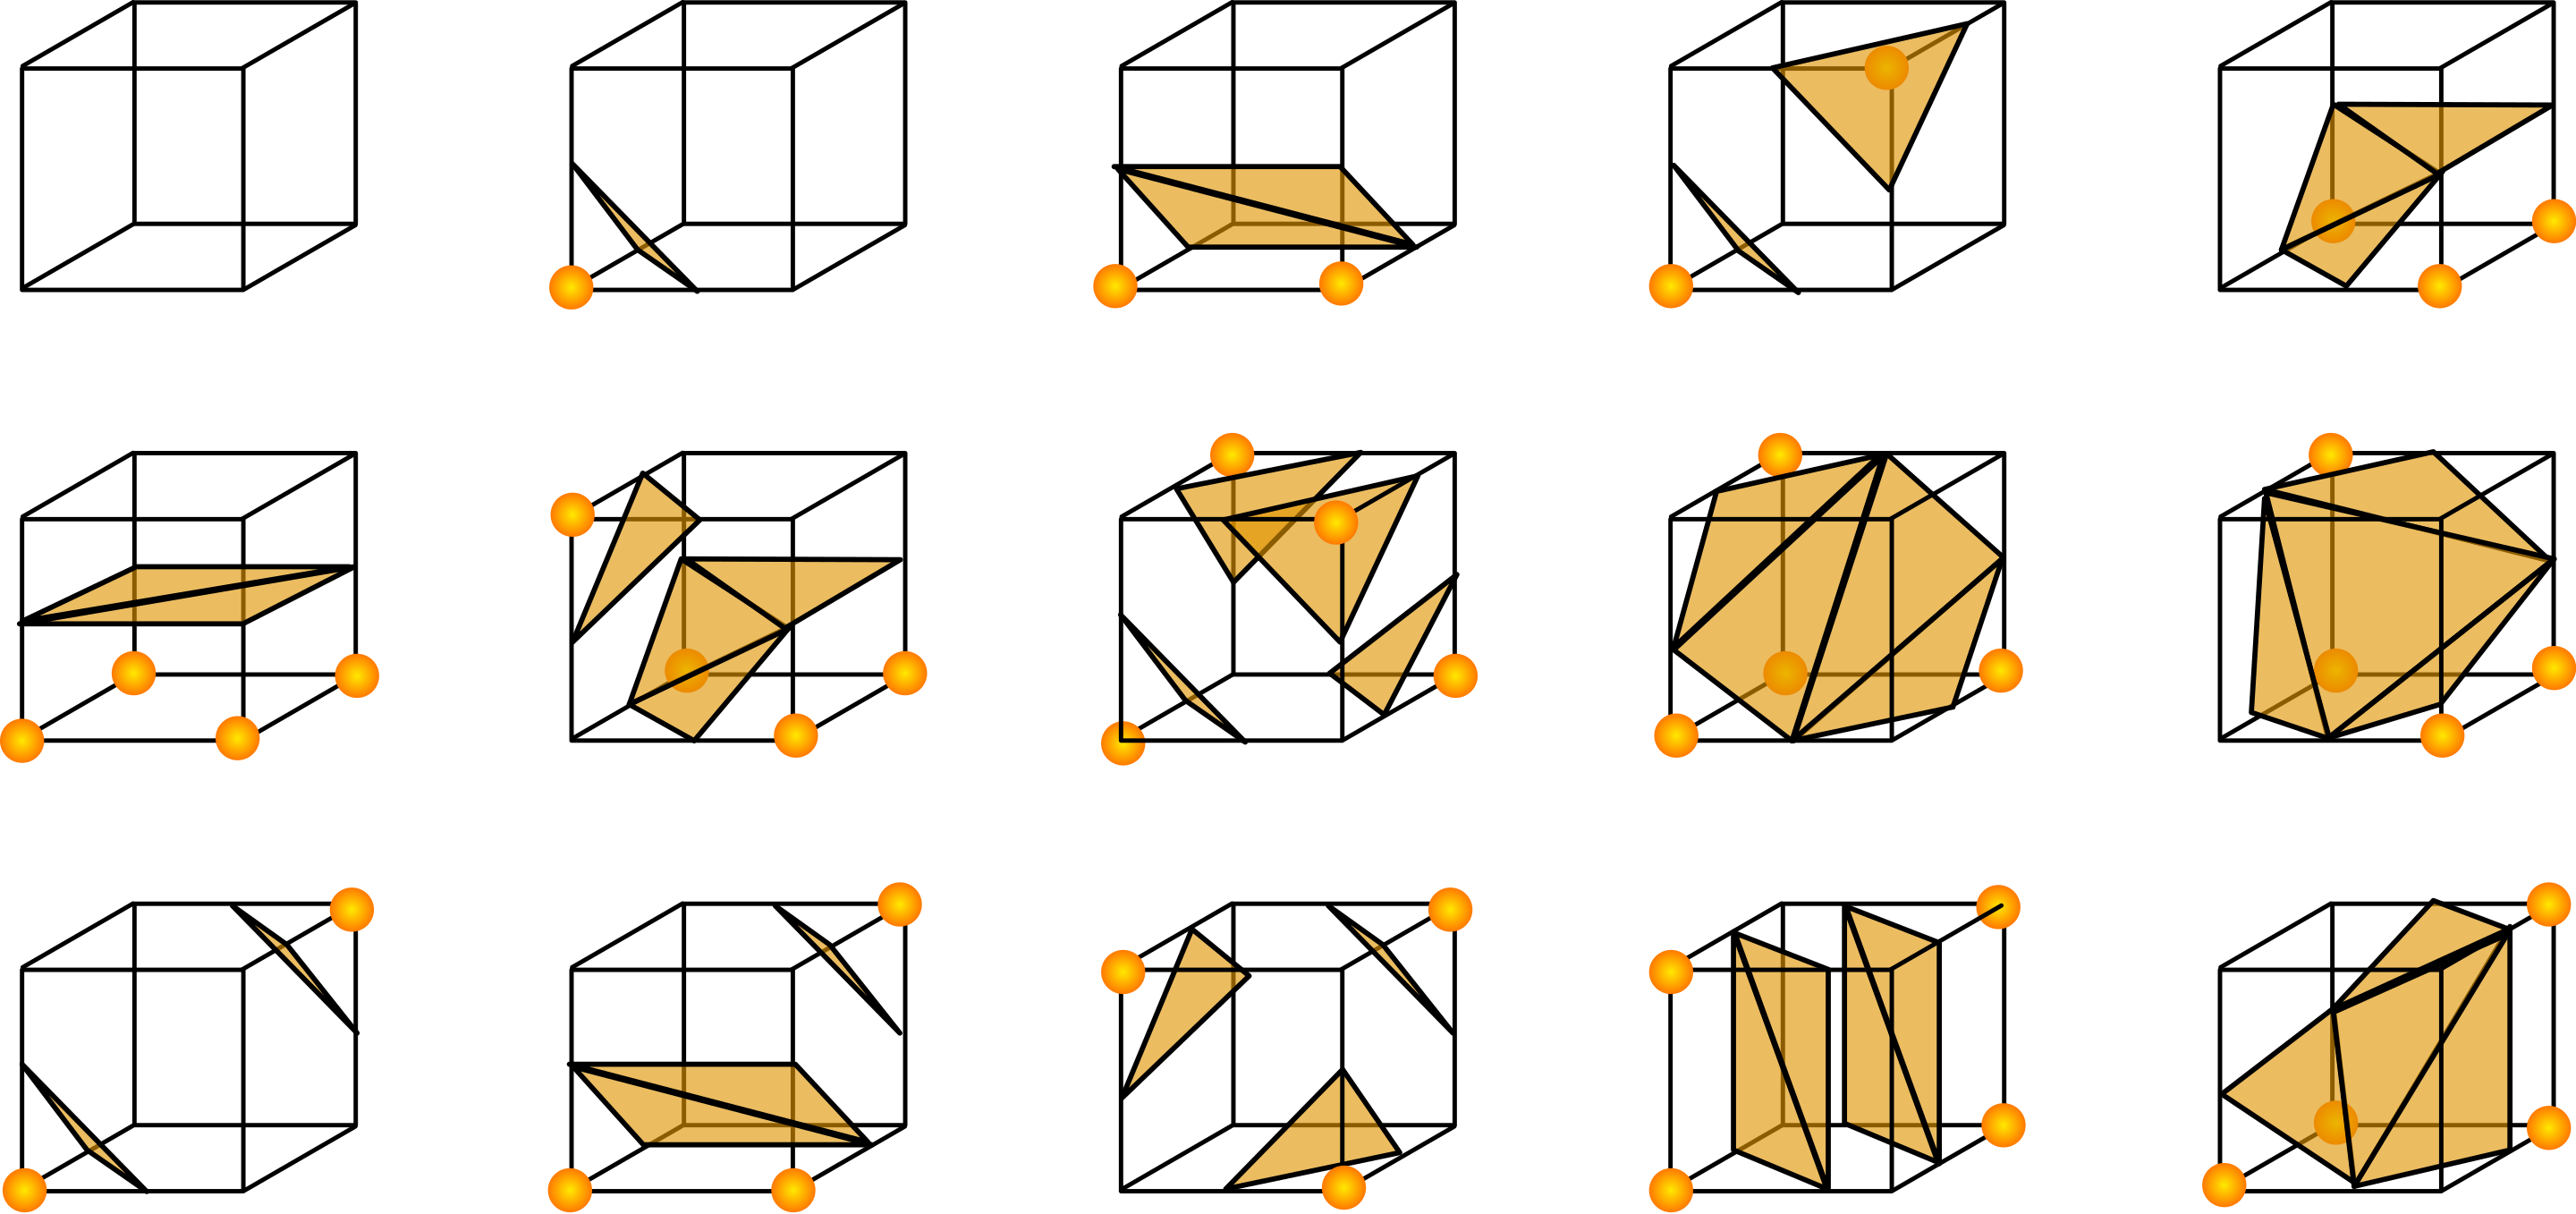
\includegraphics[width=12cm]{MarchingCubesPng}
    \caption{15 of the 256 cases for each cube. The colored vertices are the ones inside the fluid. The orange triangles are the results generated for each cube. Image courtesy of the Wikipedia page on Marching Cubes. }
    \label{figure marching cubes}
\end{figure}

The triangles generated for all the cells connect together into a watertight mesh, which can be fed into the OpenGL pipeline for rendering. This project implements the Marching Cubes algorithm by using a precomputed look-up table, which maps each of the 256 cases into an array of corresponding triangle vertices.

When the triangle mesh of the fluid surface is being rendered, the normal vectors of the surface is needed. This project chooses to approximate the normal vector using the discrete gradient of the signed distance field, $\nabla \phi$. This vector represents the normal because, intuitively, $\nabla \phi$ points in the direction where $\phi$ increases the most, which is also the direction that perpendicularly points away from the liquid surface.



\begin{figure}[H]
    \centering
    
    \begin{minipage}[t]{.49\linewidth}
        \centering
        \vspace{0pt}
        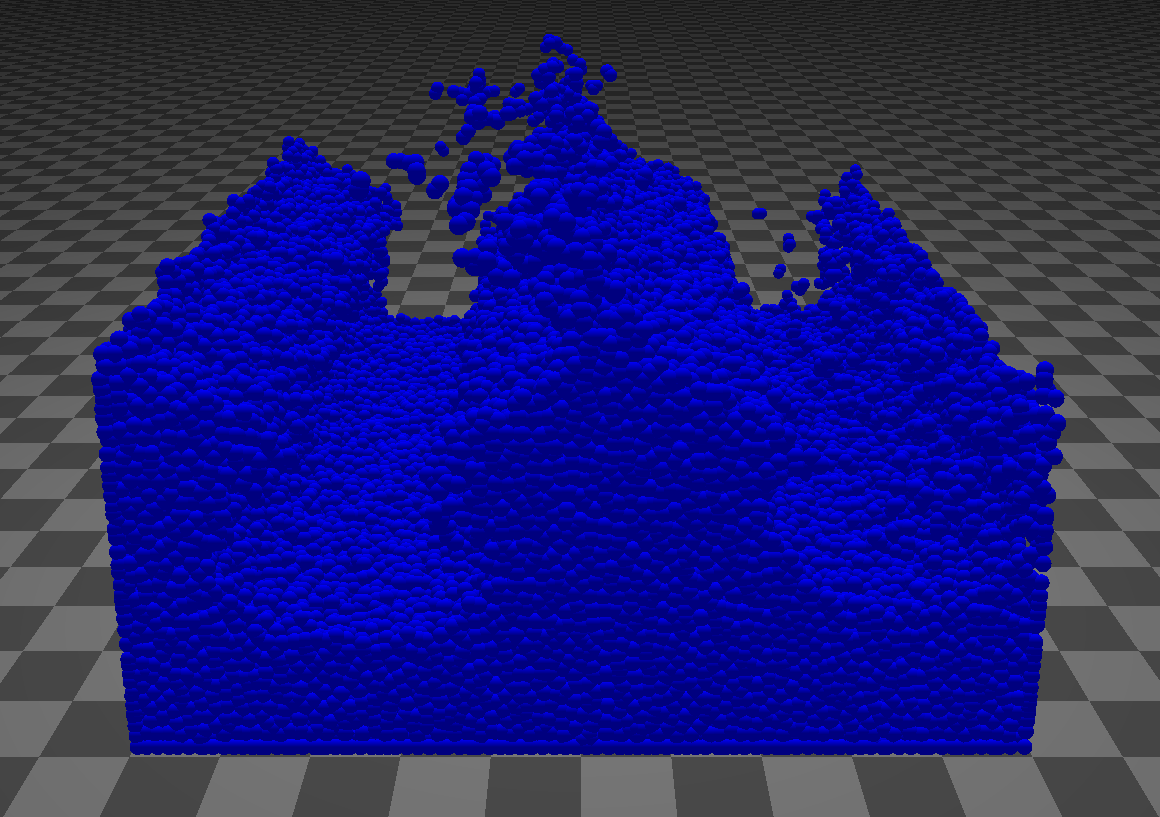
\includegraphics[width=7.4cm]{meshing_cropped/particles}
        \subcaption{PBF Particles}
    \end{minipage}
    \begin{minipage}[t]{.49\linewidth}
        \centering
        \vspace{0pt}
        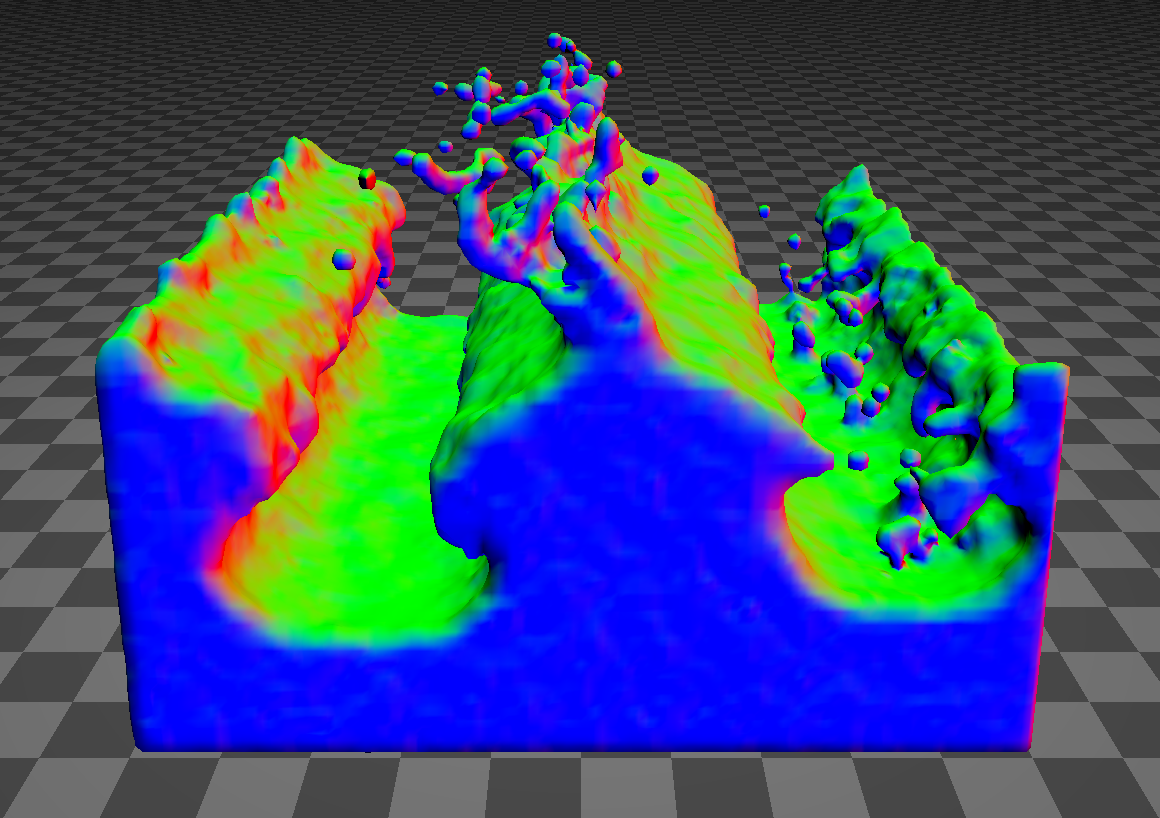
\includegraphics[width=7.4cm]{meshing_cropped/normal}
        \subcaption{Constructed mesh and its normal.\\Direction represented by colors: 
        \\ Red:$+x$ ~~ Green:$+y$ ~~ Blue:$+z$}
    \end{minipage}
    
    \caption{Surface reconstruction from particles}
    \label{figure surface reconstruction}
\end{figure}




\section{Surface Shading}

After the triangle mesh representing the liquid surface is constructed, it is put through the OpenGL pipeline for shading. The most important task falls upon the fragment shader, where the color of each pixel on the mesh is computed. In order to generate realistic coloring, it is necessary to model how rays of light interact with the liquid.

\subsection{Reflection And Refraction}
As a ray of light hits the boundary between air and liquid, part of its energy is bounced away from the surface, while the rest of enters the liquid and continues to travel inside. The two resulting rays are respectively called the \textit{reflection} and the \textit{refraction}. 

\begin{figure}[H]
    \centering
    %\includegraphics{ReflectionRefraction}
    \begin{tikzpicture}
        \filldraw[draw=LightBlue,fill=LightBlue] (-4,-3) rectangle ++(8,3);
        \draw[line width=0.5mm,blue] (-4,0) -- (4,0);

        

        \coordinate (intersect) at (0,0);

        \draw[->,-latex,line width=0.5mm] (intersect) -- (0,3) node[above](NEnd) {\large{$\textbf{N}$}};

        \draw[->,-latex,line width=0.5mm] (intersect) -- (0,-3) node[below](NEndInv) {\large{$-\textbf{N}$}};

        \draw[->,-latex,line width=0.5mm] (-2.2,2.2)node[above](inciStart){\large{$\textbf{v}_i$}} -- (intersect);


        \pic [draw, "\large{$\theta_1$}", angle eccentricity=2.0,line width=0.25mm] {angle = NEnd--intersect--inciStart};

        \draw[->,-latex,line width=0.5mm] (intersect) -- (2.2,2.2) node[above](reflEnd) {\large{$\textbf{v}_{refl}$}};

        \pic [draw, "\large{$\theta_1$}", angle eccentricity=2.0,line width=0.25mm] {angle = reflEnd--intersect--NEnd};

        \draw[->,-latex,line width=0.5mm] (intersect) -- (1.3,-2.4) node[below](refrEnd) {\large{$\textbf{v}_{refr}$}};

        \pic [draw, "\large{$\theta_{2}$}", angle eccentricity=2.5,line width=0.25mm] {angle = NEndInv--intersect--refrEnd};


        \coordinate (rightEnd) at (3.7,0);

        \node [above=0.2cm of rightEnd]{\large{$n_1$}};
        \node [below=0.2cm of rightEnd]{\large{$n_2$}};

    \end{tikzpicture}

    \caption{Reflection and Refraction.}
    \label{figure reflection refraction}
\end{figure}

Let $\textbf{v}_i$ be the direction of the incident ray, and let $\textbf{v}_{refl}$ be the direction of the reflected ray. The angle $\theta_i$ between $\textbf{v}_i$ and the surface normal $\textbf{N}$ will always be same as the angle between $\textbf{N}$ and $\textbf{v}_{refl}$. Knowing $\textbf{v}_i$ and $\textbf{N}$, $\textbf{v}_{refl}$ can be computed as:
\begin{equation}
    \label{eqn direction of reflection}
    \textbf{v}_{refl} = 2\textbf{N}(-\textbf{v}_i \cdot N) + \textbf{v}_i
\end{equation}

The direction of the refracted ray, $\textbf{v}_{refr}$, is slightly more complicated to compute. The angle $\theta_2$ between $\textbf{v}_{refr}$ and the inverse of $\textbf{N}$ is governed by the Snell's law:
$$
\frac{\sin\theta_1}{\sin\theta_2}=\frac{n_2}{n_1}
$$
where $n_1$ is the \textit{Index of Refraction} of air, and $n_2$ that of the liquid. Usually, $n_1$ is roughly equal to $1$, and the $n_2$ for water is around $1.333$. Based on Snell's law, Bec\cite{bec1997faster} derived a fast formula for computing $\textbf{v}_{refr}$:
\begin{equation}
    \label{eqn direction of refraction}
    \begin{aligned}
        \textbf{v}_{refr} &= (w-k)\textbf{N} + n\textbf{v}_{i}\mbox{~~~~ where}\\
        n &= \frac{n_1}{n_2}\\
        w &= n(-\textbf{v}_i \cdot N) \\
        k &= \sqrt{1+(m-n)(m+n)} 
    \end{aligned}
\end{equation}
Besides the direction of the reflected and refracted ray, it's also necessary to know the ratio of the incident energy that is reflected. Let this ratio be $F$, then, due to conservation of energy, the ratio of the refracted light must be $1-F$. The exact value of $F$ is determined by the Fresnel equation, which is also dependent on the polarization and spectral distribution of the light. Due to the complexity of these equations, real time computer graphics applications often use an approximation given by Schlick\cite{schlick1994inexpensive}:
\begin{equation}
    \label{eqn Schlick}
    \begin{aligned}
        F &= F_0 + (1-F_0)(1-(-\textbf{v}_i \cdot \textbf{N}))^5\mbox{~~~,where}\\
        F_0 &= \left(\frac{n_2-n_1}{n_2+n_1}\right)^2
    \end{aligned}
\end{equation}


In the OpenGL fragment shader, the final out put color will be $F$ multiplied by the color of the reflection, and $1-F$ multiplied by the color of the refraction. The reflected color is straightforward to compute, by tracing the ray in the direction of $\textbf{v}_{refl}$. However, for the refracted ray, because its path lies within the liquid, it's necessary to consider the behavior of the light ray within a colored medium. To make things more complicated, since this project supports simulating multiple phases of fluids, different fluids of different color could be mixed together in the same region. This is explored in the next subsection.

\subsection{Multiple Fluids Rendering}
\label{subsection multiphase render}
As a ray of light travels past a region of colored liquid, the energy of the light ray diminishes as a result of scattering and absorption by the liquid particles. This process is quantified by the \textit{Beer-Lambert Law}, which defines the ratio $T_r$ of the light that remains after it travels through the fluid region:
\begin{equation*}
    \begin{aligned}
        T_r &= e^{-\tau} \mbox{~~~where}\\
        \tau &= \int_0^{d} \sigma_t(\textbf{o}+x\textbf{v}) dx
    \end{aligned}
\end{equation*}
In this formula, $\textbf{o}$ is the point where the ray enters the liquid, $\textbf{v}$ its direction of travel, and $d$ the length of the path of the ray inside the water. The function $\sigma_t(\textbf{x})$ indicates how much of the light becomes extinct at location $\textbf{x}$, and the integral of the extinction across the entire path is $\tau$, the \textit{optical thickness}.

For a fluid consisting of only one type of fluid, the parameter $\sigma_t$ stays constant, so $\tau$ can be computed simply as $d\sigma_t$. However, in a region where multiple fluids are mixed together, the integral must be explicitly evaluated, usually numerically.

Moreover, the extinction parameter $\sigma_t$ is highly dependent on the wavelength of the light, which is exactly the cause for different fluids to have different color. For example, a red liquid has the lowest $\sigma_t$ for the wavelength of red, thereby allowing more red light to pass through. As a result, the numerical integration of $\tau$ needs to be performed for each of the RGB channels.

A frequently used method for computing $\tau$ is \textit{ray marching}, where the ray in question is progressed a small step at a time, accumulating the extinction along the way. Alternatively, this project invented a novel algorithm for accumulating $\sigma_t$, which is more efficient and directly makes use of the FLIP particles, which carry the concentration information:
\begin{enumerate}
    \item 
    Create a texture image, where each color channel in the texture will correspond to the thickness of a specific fluid phase. Note that this limits the maximum number of different fluids to 4.

    \item 
    Configure OpenGL's compositing step (see section \ref{section opengl}) to perform simple addition for overlapping pixels. This means that, if a pixel is covered by more than one particles, the results from rendering those particles will be added together to form the final result. On the GPU, compositing is not computed by ALUs, but hardware accelerated by a dedicated unit called the ROP(Render Output Unit).

    \item 
    Render the FLIP particles and direct the output to the texture created in step 1. For each fluid particle $p$, and for each fluid phase $f$, render the concentration of $f$ that $p$ carries into the channel designated for $f$. The configuration from step 2 will ensure that the concentrations for all particles are accumulated.

    \item 
    While rendering the mesh, at each pixel, sample the concentration texture, and use the accumulated concentration to determine $\tau$. The correct coloring can then be computed.
    
\end{enumerate}
Example results of the intermediary render stages is shown in this figure:
\newpage

%\begin{changemargin}
    
\addtolength{\topmargin}{-.875in}

\begin{figure}[H]
    \centering
    \begin{minipage}[t]{.65\linewidth}
            \vspace{0pt}
            \centering
            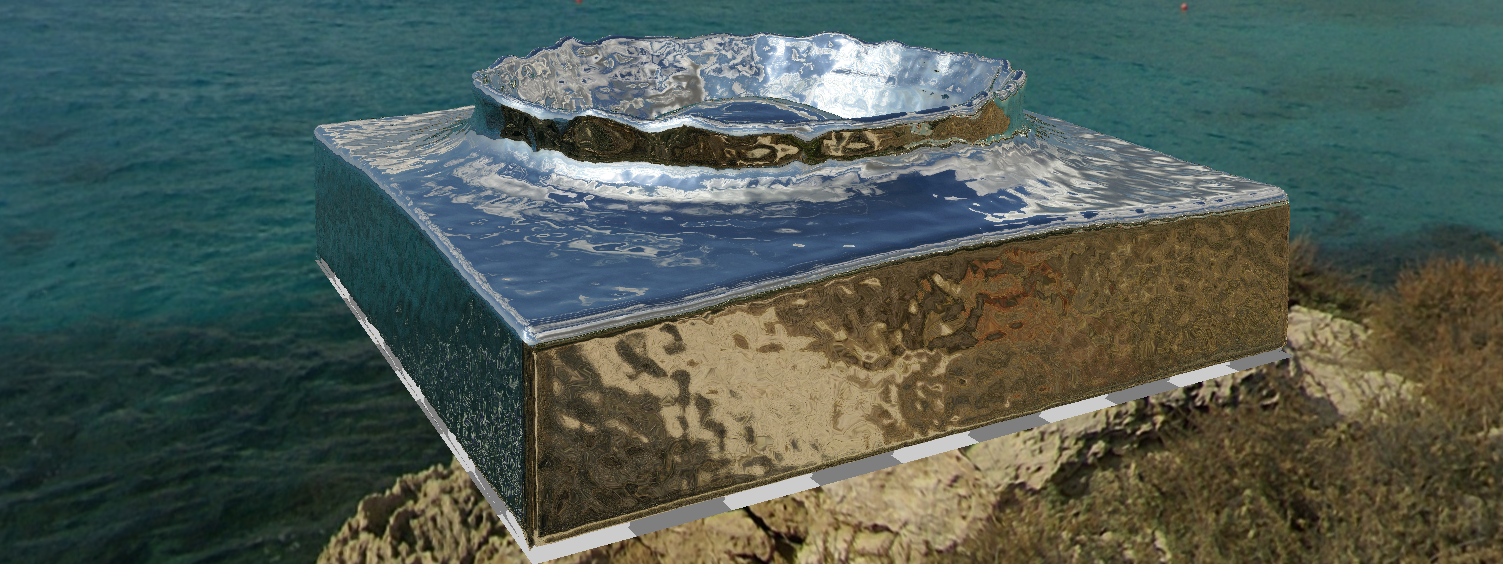
\includegraphics[width=10cm]{volume_cropped/reflection.png}
            \subcaption{The reflection}
    \end{minipage}
    
    \hspace{2pt}

    \begin{minipage}[t]{.65\linewidth}
            \vspace{0pt}
            \centering
            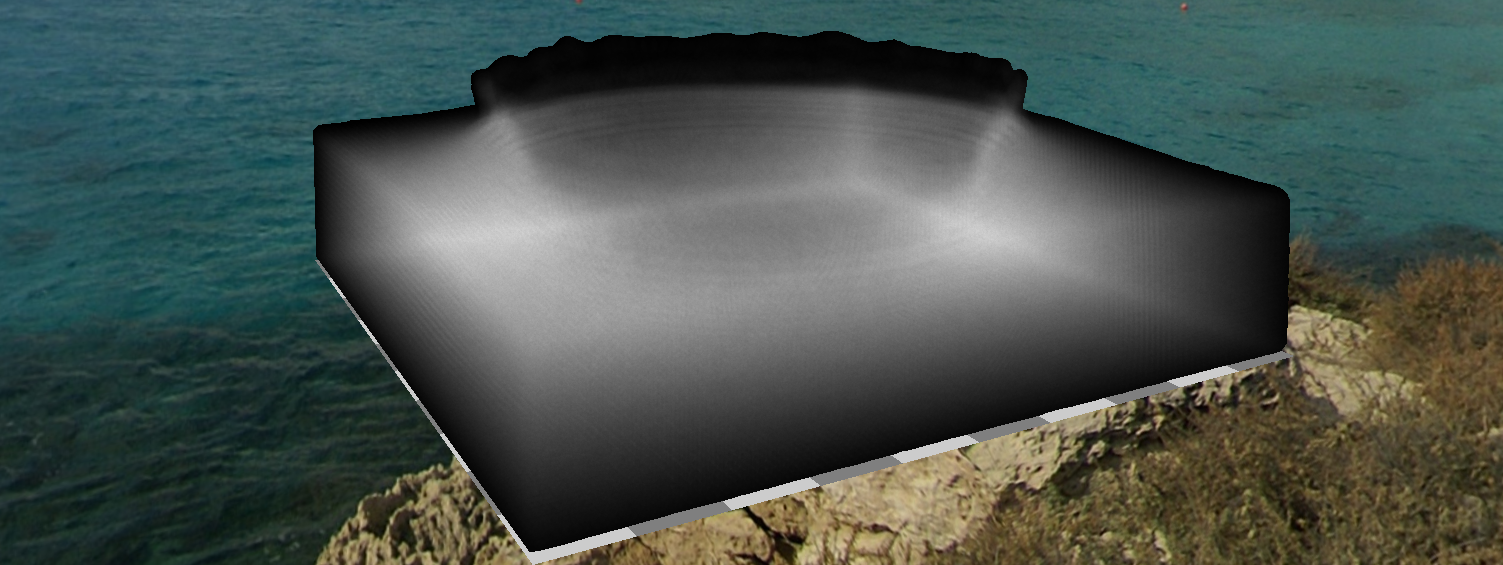
\includegraphics[width=10cm]{volume_cropped/blue.png}
            \subcaption{The thickness texture of the blue liquid. \\Brighter color indicates greater thickness.}
    \end{minipage}

    \hspace{2pt}
    
    \begin{minipage}[t]{.65\linewidth}
            \vspace{0pt}
            \centering
            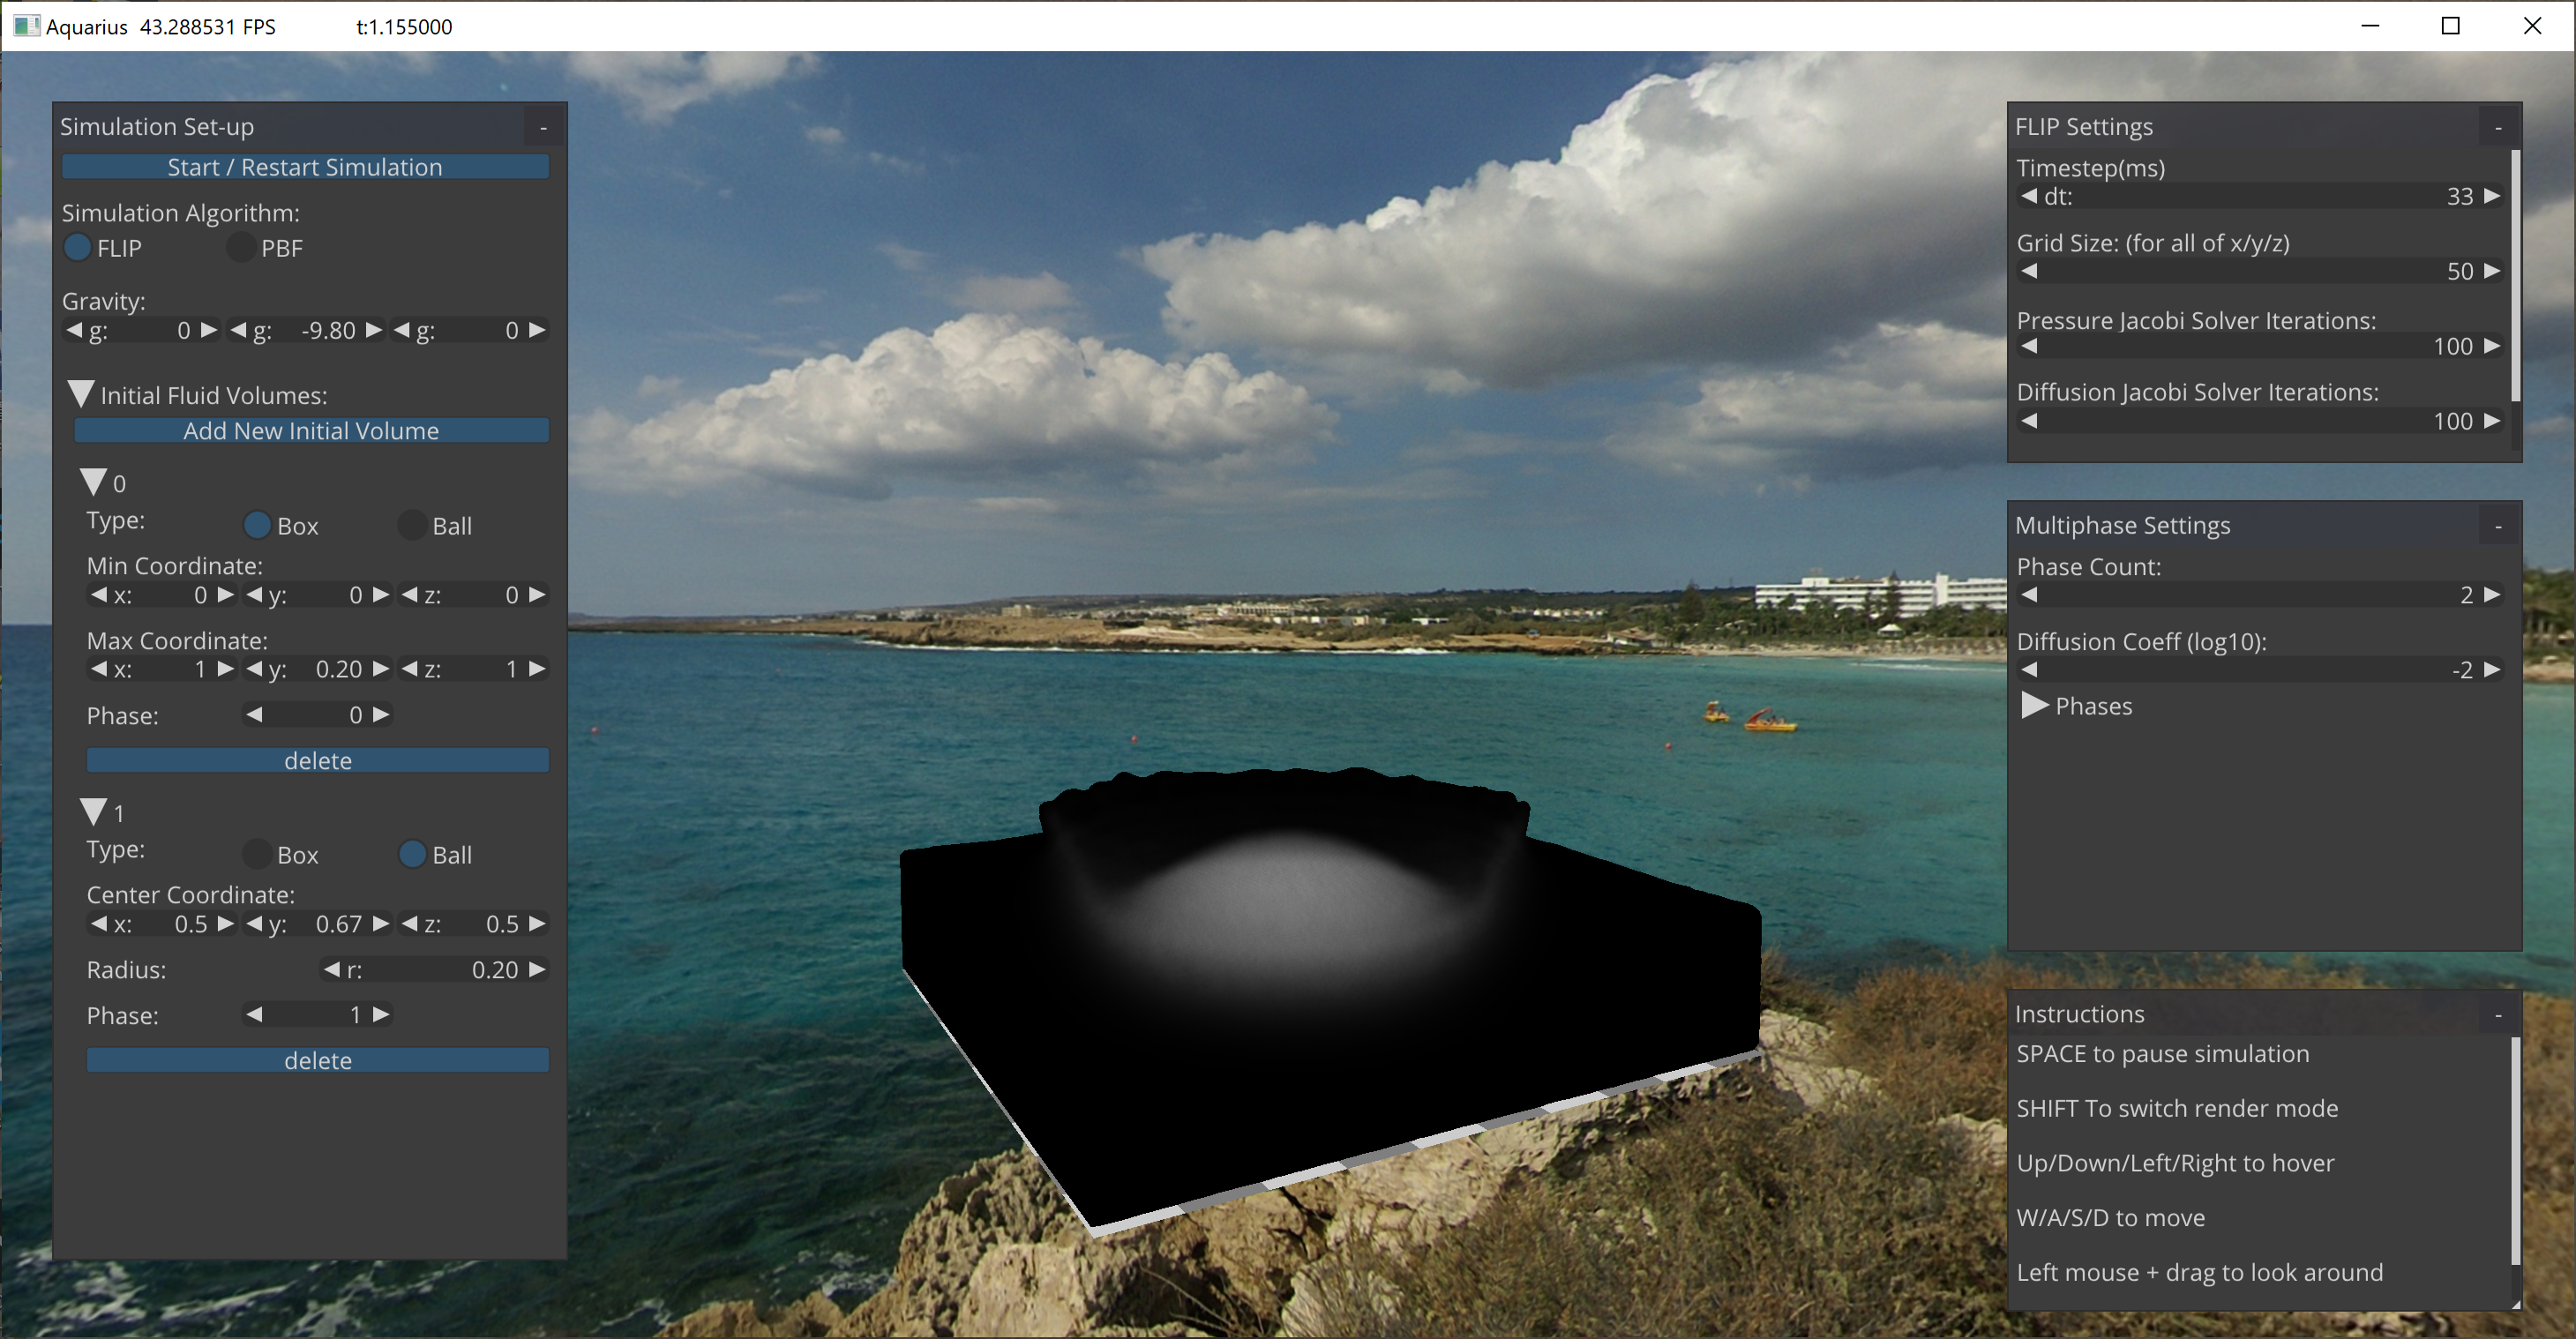
\includegraphics[width=10cm]{volume_cropped/red.png}
            \subcaption{The thickness texture of the red liquid}
    \end{minipage}

    \hspace{2pt}
            
    
    \begin{minipage}[t]{.65\linewidth}
            \vspace{0pt}
            \centering
            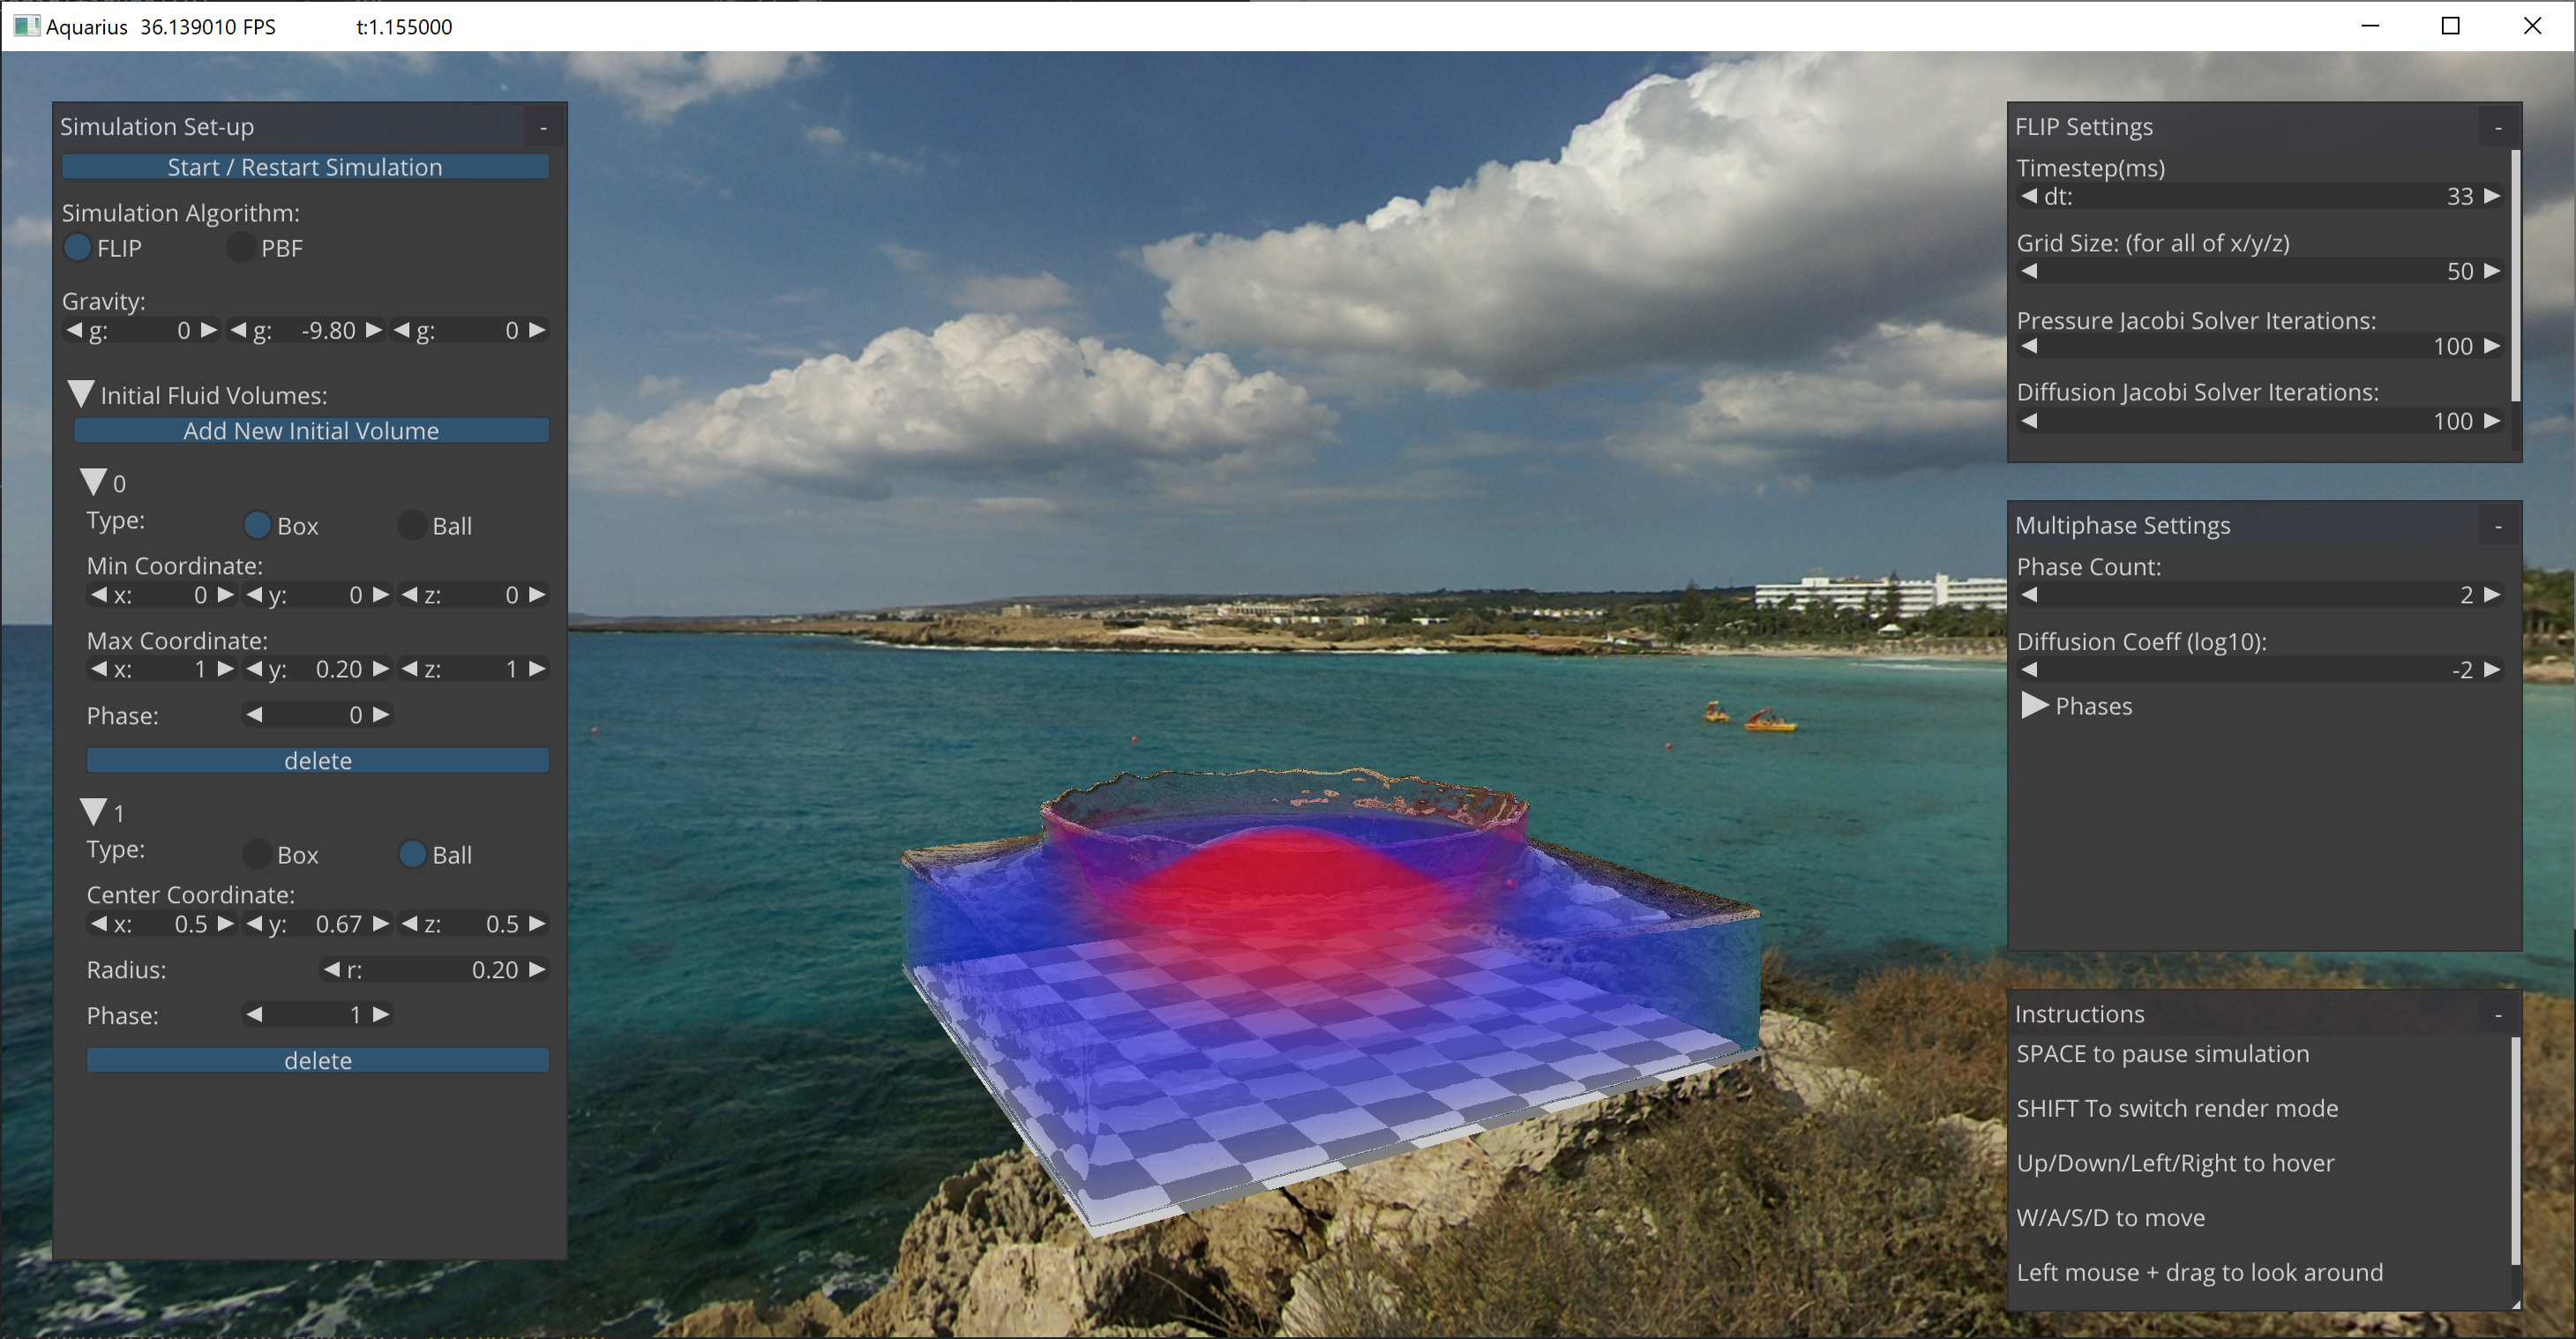
\includegraphics[width=10cm]{volume_cropped/refraction.png}
            \subcaption{The refraction color.}
    \end{minipage}

    \hspace{2pt}

    \begin{minipage}[t]{.65\linewidth}
            \vspace{0pt}
            \centering
            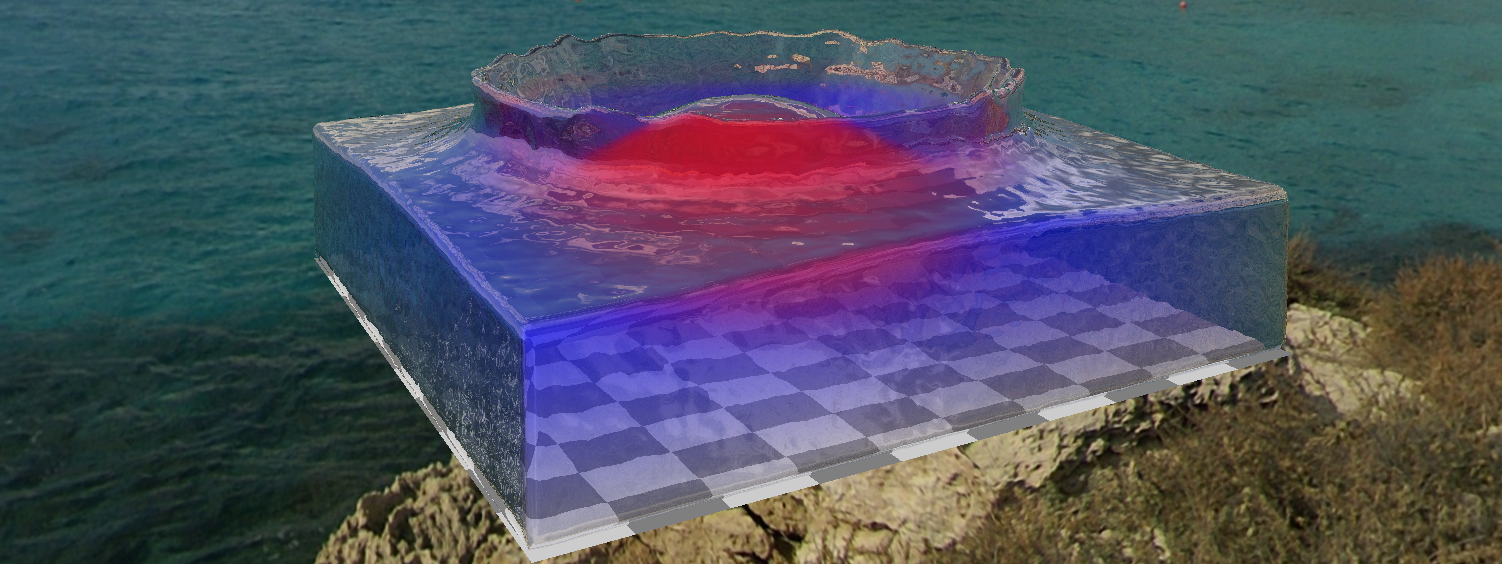
\includegraphics[width=10cm]{volume_cropped/final.png}
            \subcaption{Final result}
    \end{minipage}

    \hspace{2pt}
            

    \caption{Intermediary and final outputs of the renderer. The images show the moment after a large ball of red liquid falls into a box of blue liquid}
    \label{figure volume render}
\end{figure}


%\end{changemargin}
\addtolength{\topmargin}{.875in}
